\documentclass{article}
\usepackage{graphicx}
\usepackage{amssymb}
\usepackage{float}
\usepackage{hyperref}
\begin{document}

\title{Reactor Simulator: Transport Theory}

\author{Nicholas F. Herring\\
North Carolina State University\\
\href{mailto: nfherrin@ncsu.edu}{\texttt{nfherrin@ncsu.edu}}
}

\date{August 2017}

\maketitle

%RAY TRACING THEORY SECTION!!!!!!!!!!!!!!!!!!!!!!!!!!
%!!!!!!!!!!!!!!!!!!!!!!!!!!!!!!!!!!!!!!!!!!!!!!!!!!!!!!!!!!!!!!!!!!!!!!!!!
%!!!!!!!!!!!!!!!!!!!!!!!!!!!!!!!!!!!!!!!!!!!!!!!!!!!!!!!!!!!!!!!!!!!!!!!!!
\section{Ray Tracing Theory}
%CELL NUMBERING METHOD SUBSECTION!!!!!!!!!!!!!!!
%!!!!!!!!!!!!!!!!!!!!!!!!!!!!!!!!!!!!!!!!!!!!!!!!!!!!!!!!!!!!!!!!!!!!!!!!!
\subsection{Cell Numbering Method}

The method of cell numbering in the program is based off of four different parameters.

\begin{enumerate}
\item Radial section number $l=1, 2, 3, \dots, L$
\item Octant number $i=1, 2, 3, \dots, 8$
\item Pincell ``column" number $n=1, 2, 3, \dots, N$
\item Pincell ``row" number $m=1, 2, 3, \dots, M$
\end{enumerate}

The total cell number is determined by the following equation:
\begin{equation}
 c=i+8(l-1)+8 L(n-1)+8 LN(m-1)
 \label{eq:cellnumber}
\end{equation}

Figure \ref{fig:pincell} shows the numbering system of the first pincell in action. 
The cells are numbered from the bottom left outside of the pin cell, circling clockwise and going inward.

\begin{figure}[H]
\begin{center}
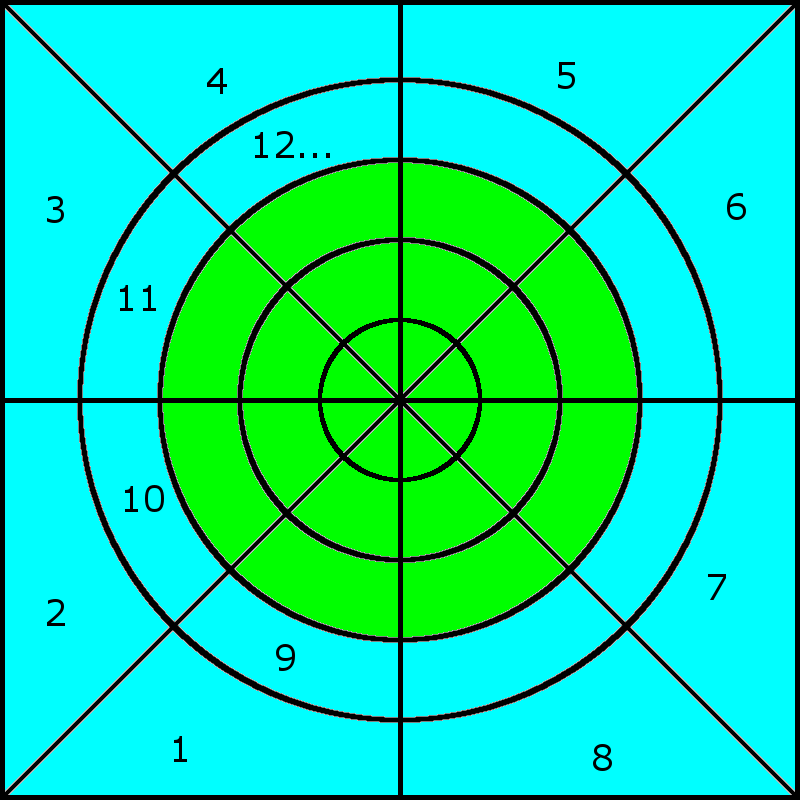
\includegraphics[width=40mm]{pincell.png}
\end{center}
\caption{Pincell numbering system}
\label{fig:pincell}
\end{figure}

Figure \ref{fig:pingrid} shows the numbering system for the assembly of pins. 
The value of the row number goes upwards from 1 at the bottom. 
The column number goes right from 1 at the far left.

\begin{figure}[H]
\begin{center}
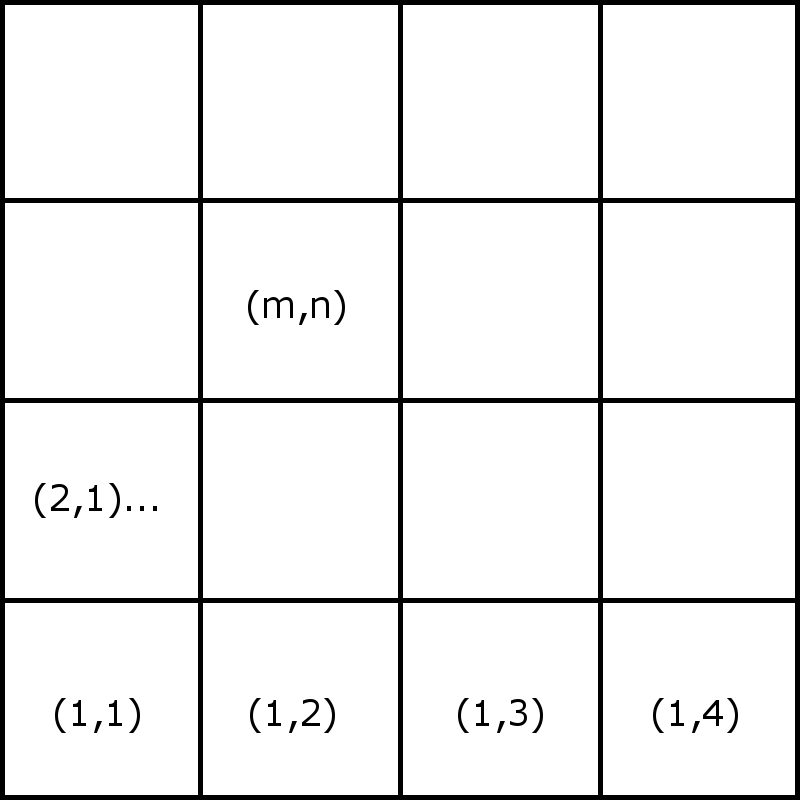
\includegraphics[width=40mm]{pingrid.png}
\end{center}
\caption{Assembly Numbering System}
\label{fig:pingrid}
\end{figure}

Pins are assumed to all be square with a user defined width of $\Delta$. 
Each pin is divided into $L$ radial sections, which means it has $L-1$ dividing circles of radius $r_l$ for $l=1,2,\dots,L-1$ where $r_L=0$ and $r_0=\infty$ by definition.

%DETERMINING CELL NUMBER SUBSECTTION!!!!!!!!!!!
%!!!!!!!!!!!!!!!!!!!!!!!!!!!!!!!!!!!!!!!!!!!!!!!!!!!!!!!!!!!!!!!!!!!!!!!!!
\subsection{Determining the Cell Number Containing a Point}

Define $A$ as the physical domain of the problem, such that $A$ represents all points $(x,y)$ on the open interval
\begin{center}
$[0< x< N\Delta \land 0< y< M\Delta]$
\end{center}
Also define the boundary of $A$ as $\delta A$ so that $(x,y)\in \delta A$ is such that
\begin{center}
$[(0\leq x\leq N\Delta \land y\in \{0,M \Delta\}) \lor (0\leq y\leq M\Delta \land x\in \{0,N \Delta\})]$
\end{center}

For a point $(x,y)\in A$, the cell that $(x,y)$ belongs to can be determined as follows.

To determine the grid ``column'' the following equation is solved for the integer $n$:
\begin{equation}
\Delta (n-1)<x<\Delta n
\label{eq:nsolution}
\end{equation}

To determine the grid ``row'' the following equation is solved for the integer $m$:
\begin{equation}
\Delta (m-1)<y<\Delta m
\label{eq:msolution}
\end{equation}

To simplify when determining the radial number $l$ and the octant number $i$, the location variables $(x,y)$ are transformed to $(\tilde{x},\tilde{y})$ by a coordinate transform to make the pincell $(m,n)$, that point $(x,y)$ belongs to, centered about the transformed coordinate system's origin, $(0,0)$. 
This is done by the following equations:
\begin{equation}
\tilde{x}=x-\Delta (n-1/2)
\label{eq:xtransform}
\end{equation}
\begin{equation}
\tilde{y}=y-\Delta (m-1/2)
\label{eq:ytransform}
\end{equation}

After this transform has been applied, the radial cell $l$ can be determined by solving the following equation for the integer $l$:
\begin{equation}
r_l<\sqrt{\tilde{x}^2+\tilde{y}^2}<r_{l-1}
\label{eq:lsolution}
\end{equation}

The determination of the octant number is slightly more complicated, and is solved by the following elimination logic:

\vspace{5mm}
\texttt{If} $\frac{|\tilde{x}|}{|\tilde{y}|} > 1$ \texttt{then}

\qquad $i\ne 2, 3, 6, 7$

\texttt{else}

\qquad $i\ne 1, 4, 5, 8$

\texttt{If} $\tilde{x} > 0$ \texttt{then}

\qquad $i\ne 1, 2, 3, 4$

\texttt{else}

\qquad $i\ne 5, 6, 7, 8$

\texttt{If} $\tilde{y} > 0$ \texttt{then}

\qquad $i\ne 1, 2, 7, 8$

\texttt{else}

\qquad $i\ne 3, 4, 5, 6$
\begin{equation}
\label{eq:isolution}
\end{equation}

With equations \ref{eq:nsolution}--\ref{eq:isolution}, the proper value of the actual cell number $c$ can be determined by equation \ref{eq:cellnumber}. 
Note here that any point $(x,y)\notin A$ is assigned the default cell number $c=-1$.

%STEP CONVERGENT RAY TRACING SUBSECTTION!!
%!!!!!!!!!!!!!!!!!!!!!!!!!!!!!!!!!!!!!!!!!!!!!!!!!!!!!!!!!!!!!!!!!!!!!!!!!
\subsection{Step Convergent Ray Tracing}

With the ability to determine which cell a point $(x,y)$ is in, the ray can now be traced by stepping along the characteristic curves. 
These curves are started from the edges of the domain with discrete angles determined by the chosen quadrature set of form $(\gamma_k,\theta_k,\omega_k)$ for $k=1,2,\dots,K$. Where $0<\gamma_k<180$, $0<\theta_k<90$, and $\sum_{k=1}^K\omega_k=2\pi$. 
The coordinate system associated with these angles is shown in Figure \ref{fig:anglecords}:

\begin{figure}[H]
\begin{center}
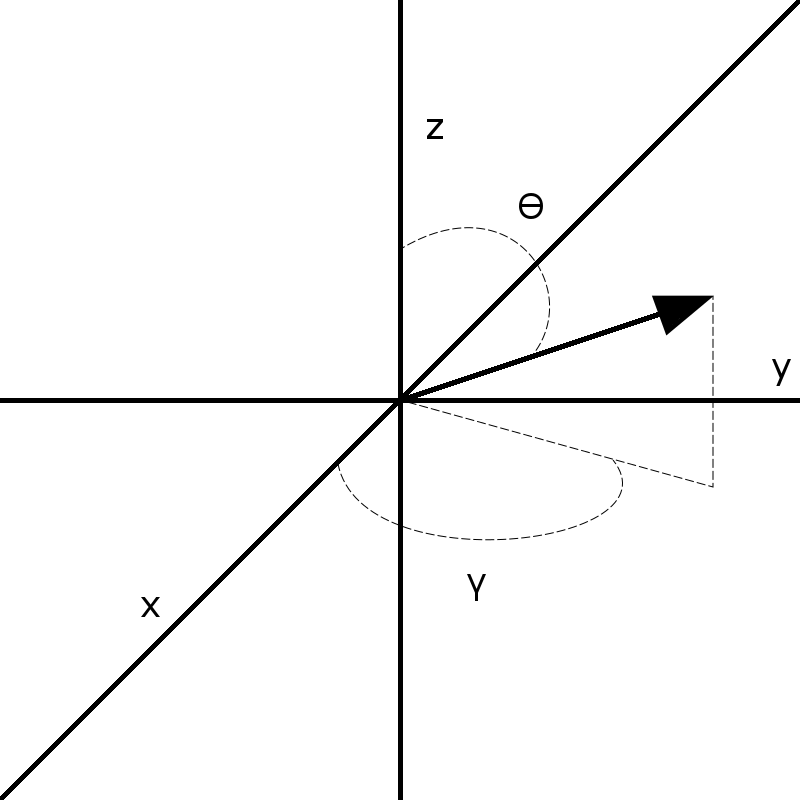
\includegraphics[width=40mm]{coordinates.png}
\end{center}
\caption{Angle Coordinates System}
\label{fig:anglecords}
\end{figure}

The rays are begun at points separated by the ray width $h$ along a line orthogonal to the characteristic curves (note that it is required here that $\Delta~ /h \in~ \mathbb{Z}$). 
The rays are started from the left, right, and bottom sides of the domain. 
Left and bottom for $\gamma>90$, and right and bottom for $\gamma<90$. 
A trivial proof, not to be repeated here, shows the spacing along the side can be calculated geometrically. For the curves starting on the left side, the spacing $s$ between the starting points along $\delta A$ is given by:
\begin{equation}
s=\frac{h}{\cos({\gamma})}
\label{eq:leftpsacing}
\end{equation}

For curves starting from the right side, the spacing $s$ is given by:
\begin{equation}
s=\frac{h}{-\cos({\gamma})}
\label{eq:rightspacing}
\end{equation}

For curves starting from the bottom side, the spacing $s$ is given by:
\begin{equation}
s=\frac{h}{\sin({\gamma})}
\label{eq:botspacing}
\end{equation}

The first starting point, $(x_s^1,y_s^1)$, for a given angle $(\gamma_k,\theta_k,\omega_k)$ is determined by the value of $\gamma_k$. 
For $\gamma_k<90$, the first ray's start point is determined by the following equation:
\begin{equation}
(x_s^1,y_s^1)=(0,M\Delta -\frac{s}{2})
\label{eq:lt90first}
\end{equation}

For $\gamma_k>90$, the first ray's start point is determined by the following equation:
\begin{equation}
(x_s^1,y_s^1)=(N\Delta,M\Delta -\frac{s}{2})
\label{eq:gt90first}
\end{equation}

After the first ray start points are properly determined by equations \ref{eq:lt90first} or \ref{eq:gt90first}, the next ray begins at the point $(x_s,y_s) = (x_s^1,y_s^1-s)$. 
This trend is continued with starting locations, until eventually $y_s<0$.
At this point the locations must now start from the bottom of the domain, $y_s=0$. 
However, the orthogonal spacing $h$ between each characteristic MUST BE PRESERVED!
In order to achieve this spacing, the first ray started along the bottom edge of the domain must be spaced from the side that the previous ray was started at by the special spacing $\tilde{s}$.
Where $y_s^f$ is the $y$ value of the final starting point on either the left or right side. For curves starting on the left side:
\begin{equation}
\tilde{s}=\frac{s-y_s^f}{\tan(\gamma)}
\label{eq:firstbotspace}
\end{equation}

For curves starting on the right side:
\begin{equation}
\tilde{s}=\frac{s-y_s^f}{\tan(180-\gamma)}
\label{eq:secondbotspace}
\end{equation}

The actual definition of the characteristic curve for a given start point $(x_s,y_s)\in \delta A$ and angle $(\gamma_k,\theta_k,\omega_k)$ is the set of points $(x,y)\in A$ along 
\begin{equation}
y=y_s+\tan{(\gamma_k)}(x-x_s)
\label{eq:curvedef}
\end{equation}

Upon beginning a ray trace, the cell start point, $(x_b,y_b)$, is set to $(x_b,y_b)=(x_s,y_s)$, determined by equations \ref{eq:leftpsacing}--\ref{eq:firstbotspace}. 
It is then stepped along by the step size $\xi$, with the maximum and starting value being $\xi_0=\Delta(1/4-10^4\epsilon)$, along the characteristic curve.
So the ray length $v$ becomes $v+\xi$ and the 2D point along it $(x,y)$ becomes $(x+\xi \cos{\left[\gamma\right]},y+\xi \sin{\left[\gamma\right]})$. 
Once the point along the ray reaches a new cell, i.e. $c(x_b,y_b)\ne c(x,y)$ (determined by equations \ref{eq:nsolution}--\ref{eq:isolution} being applied with equation \ref{eq:cellnumber}), the tracer steps back by half of the value of the current step size $\xi$. 
If the cell is still not the original cell it steps back again. 
It then halves the new step size before stepping forward. 

The tracer repeats this process until the step size has reached the minimum step size, defined as $\xi_{min}=10^4 \epsilon \Delta$ where $\epsilon$ is the machine precision, for double precision $\epsilon\approx10^{-16}$. 
It then it steps forward with this size until in the new cell.
Once it confirms that the point is now in a new cell, the tracer defines that point to be the point at which the new segment of the ray starts.
The tracer records the length of the ray in the old cell as $\frac{|x_e-x_b|}{\cos{(\gamma)}}$, where $x_b$ is the $x$ value of the start point of the segment and $x_e$ is the $x$ value of the end point of the segment (which should be noted is the start point of the next segment). 
Note that this is equivalent to the similarly defined value $\frac{|y_e-y_b|}{\sin{(\gamma)}}$. 
The tracer resets $\xi=\xi_0$ and $(x_b,y_b)=(x_e,y_e)$ then repeats the process. 
This is done until the start point of the next cell $(x_b,y_b)$ along the characteristic curve is such that $c(x_b,y_b)=-1$.
This process is repeated for every start point $(x_s,y_s)\in \delta A$ corresponding to a given angle  $(\gamma_k,\theta_k,\omega_k)$ separated along the starting side of the domain by the spacing $s$. 



\end{document}













